\section{Conclusion}
\begin{frame}
	\begin{center}
	%{\color{-green!15!yellow}
	\Large{Conclusion}
	%}
	\end{center}
\end{frame}


\begin{frame}
	Observations after the challenge:
	\begin{itemize}
		\item Linear models performed badly in the challenge.
		\item K Nearest Neighbors nearly beats most of the challenges benchmarks.
		\item Boosting methods and neural networks performed well.
	\end{itemize}
\end{frame}

\subsection{Results}
\begin{frame}
	\frametitle{Results}
	\begin{table}[width=\textwidth]
	\begin{tabular}{|l|c|c|}
	\hline
	Classifier & AMS & rank \\
	\hline
	Logistic Regression & 2.06934 & 1429 \\
	\hline
	k Nearest Neighbor & 3.18323 & 996 \\
	\hline
	XGBoost & 3.71268 & 65 \\
	\hline
	XGBoost original & 3.71885 & 45 \\
	\hline
	Winning submission & 3.80581 & 1 \\
	\hline
	\end{tabular}
	\caption{Performances of used methods}
	\end{table}
	\vspace{2ex}
	\begin{center}
		1785 participating teams in total.	
	\end{center}

\end{frame}

\begin{frame}
	\frametitle{Results}
	\begin{figure}
		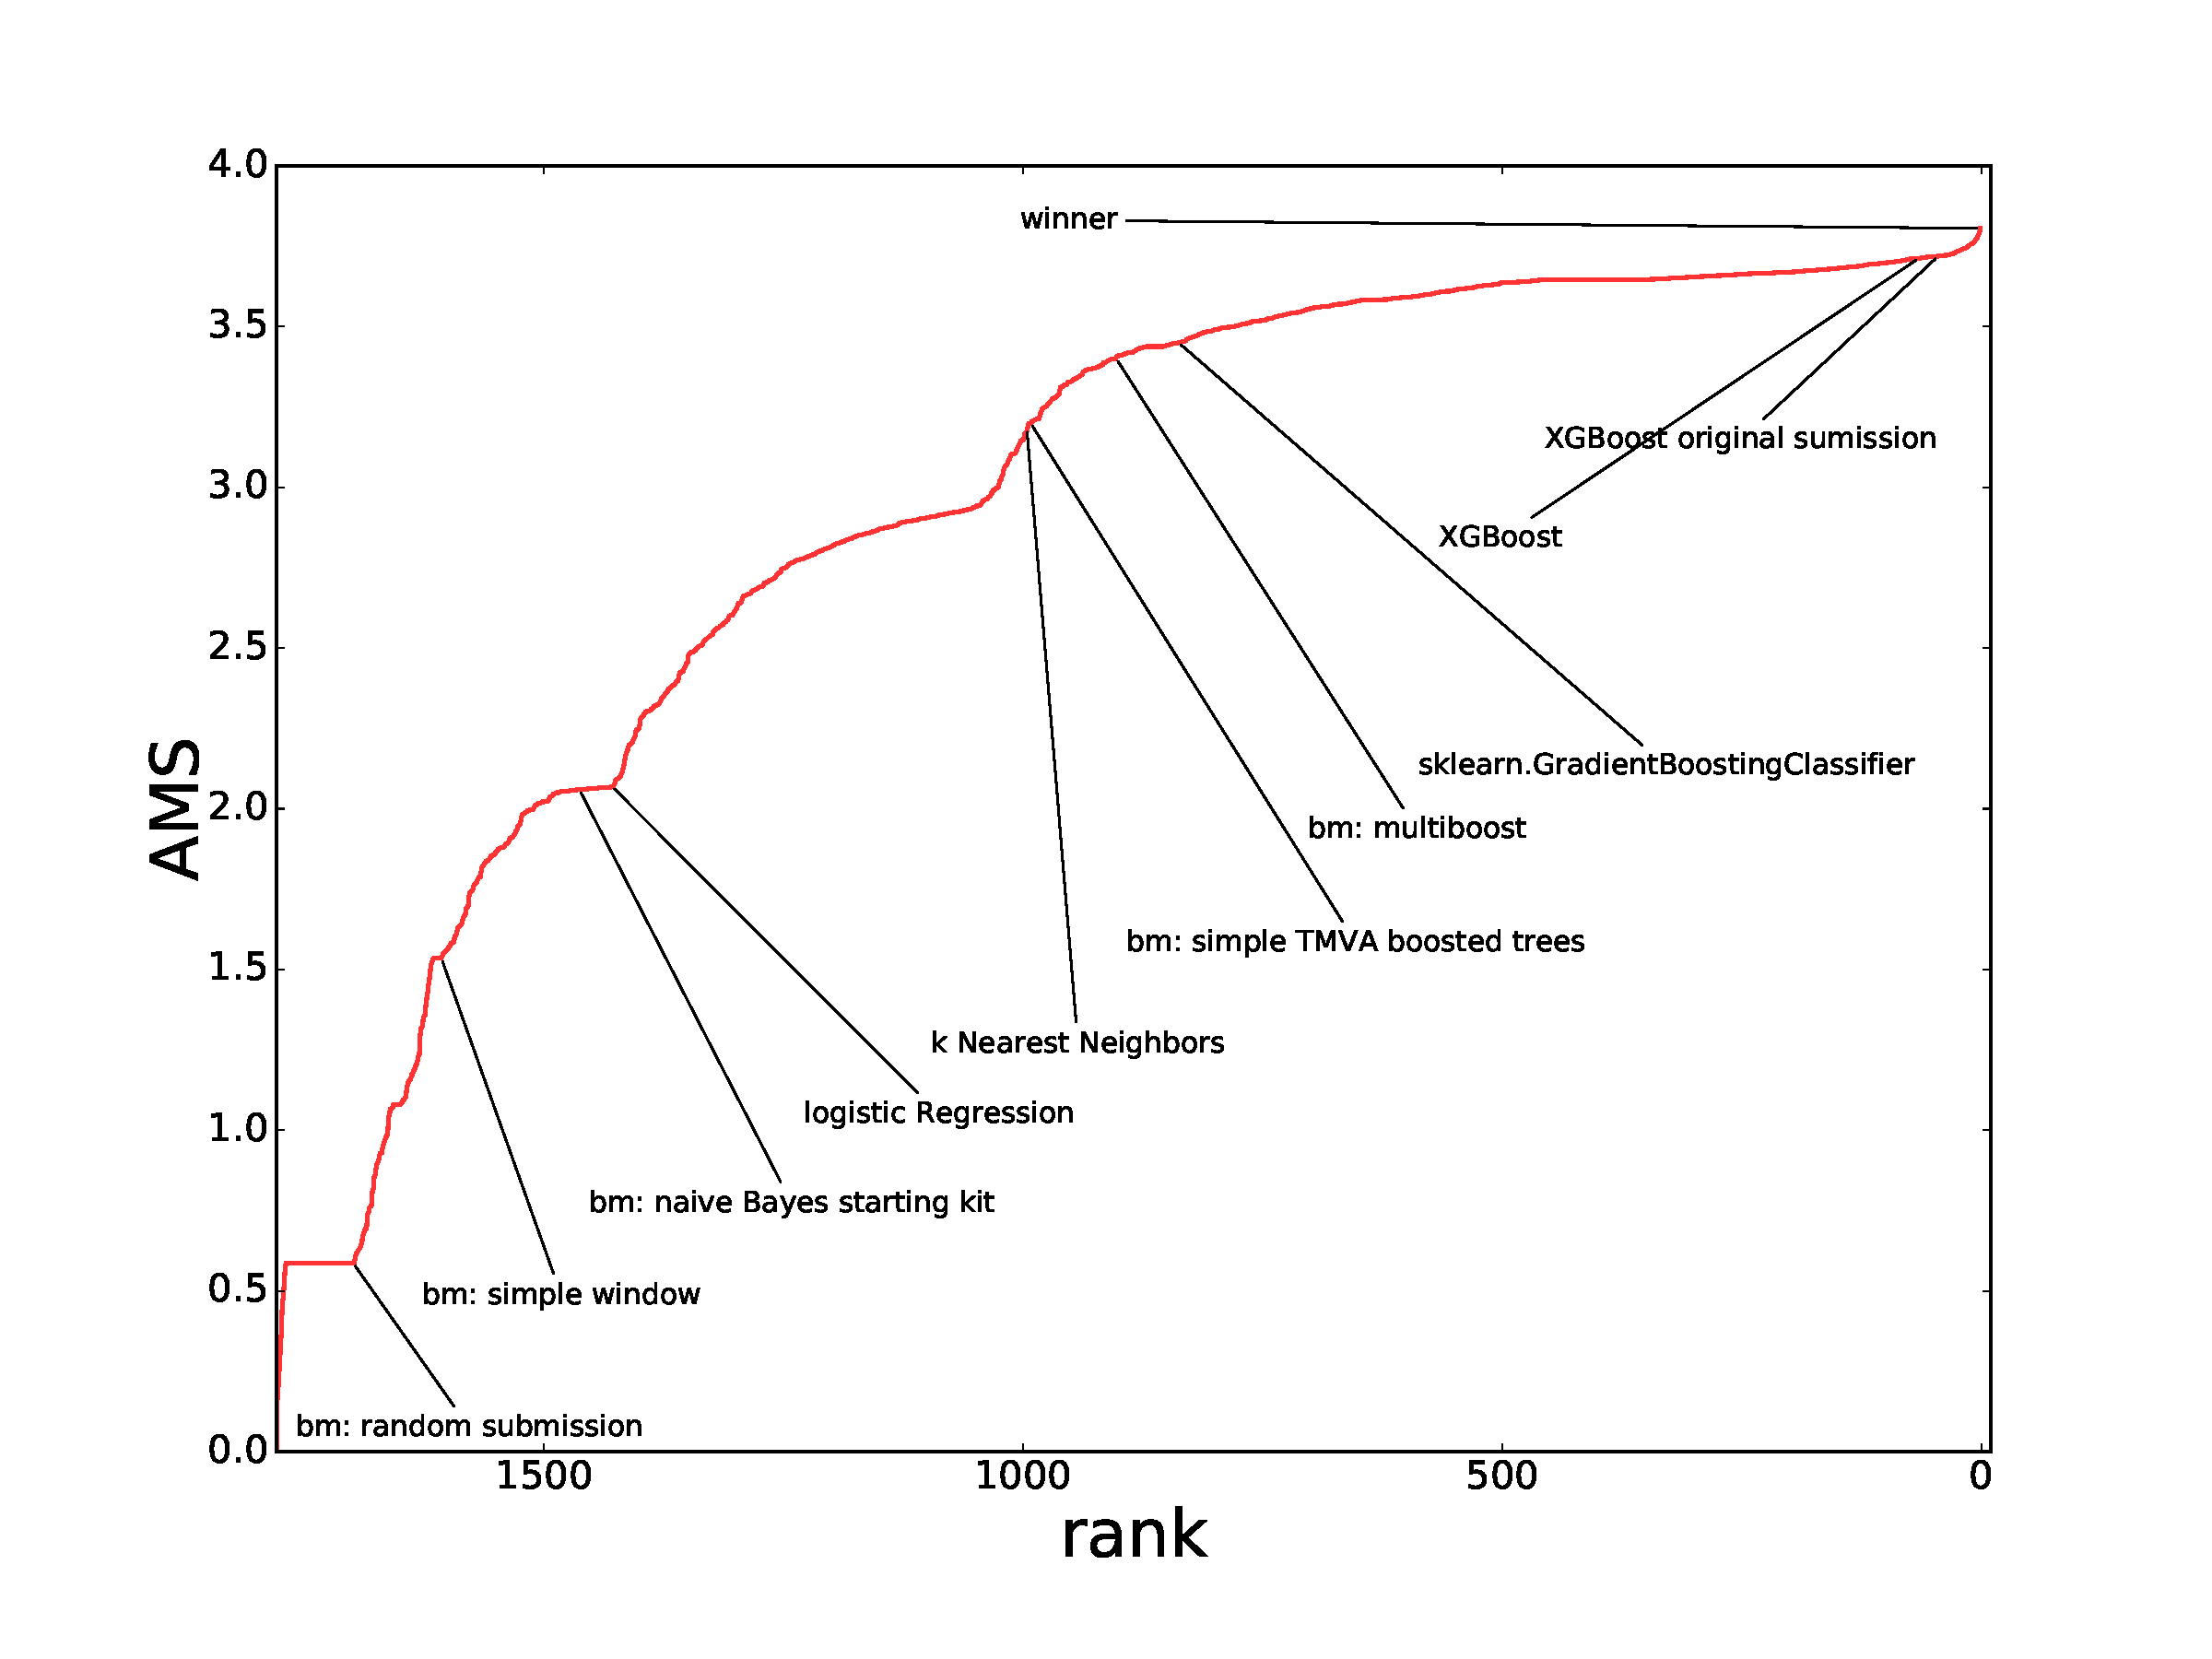
\includegraphics[trim=50 50 50 75,clip,width=0.7\textwidth]{images/amscompare}
		\caption{AMS of all final submissions in the challenge. \cite{higgsChallenge}}
	\end{figure}
\end{frame}